\documentclass[12pt]{article}

%Paquetes a utilizarse
\usepackage[width=7in, height=9.5in, top=0.75in, papersize={8.5in,11in}]{geometry}
\usepackage[spanish]{babel} 
\decimalpoint
\usepackage[utf8]{inputenc}
\usepackage{bbding}
\usepackage[colorlinks = true, linkcolor = blue, urlcolor = BlueViolet, citecolor = OliveGreen]{hyperref}
\usepackage{graphicx}
\usepackage{amssymb,amsthm,amsmath}
\usepackage{enumerate}
\usepackage{array,multicol,multirow}
\usepackage{xcolor}
\usepackage{fancybox,tcolorbox}
\usepackage{caption,subcaption,float,tabularx}
\usepackage{enumitem}

\theoremstyle{definition}
\newtheorem{corolario}{Corolario}
\newtheorem{lema}[corolario]{Lema}
\newtheorem{proposicion}[corolario]{Proposición}
\newtheorem{teorema}[corolario]{Teorema}
\newtheorem{propiedad}[corolario]{Propiedad}
\newtheorem*{observacion}{Observación}
\newtheorem{definicion}{Definición}
\newtheorem*{demostracion}{Demostración}
\newtheorem{ejemplo}{Ejemplo}
\newtheorem{problema}{Problema}
\newtheorem*{solucion}{Solución}
\newtheorem{ejercicio}{\PencilRightDown \  Ejercicio}
\newtheorem{step}{Paso}
\newtheorem{credito}{Crédito}

\usepackage{tikz}
\usetikzlibrary{arrows.meta,babel,calc,positioning}

\renewcommand{\arraystretch}{1.5}
\providecommand{\abs}[1]{\lvert#1\rvert}
\providecommand{\norm}[1]{\lVert#1\rVert}

\renewcommand{\tabularxcolumn}[1]{m{#1}}
\newcommand{\Evaluacion}[4]{
\setcounter{ejercicio}{0}
\noindent\begin{tabular}{lcr}
	\includegraphics[height=3cm]{Logos/logo-UES.png}\hspace{2.5em}
	&
	\includegraphics[height=2.75cm]{Logos/logo-PJT.png}
	& 
	\hspace{2.5em}\includegraphics[height=2.75cm]{Logos/logo-MINEDUCYT.png}
\end{tabular}

\hfill

\begin{center}
    
    UNIVERSIDAD DE EL SALVADOR
    \\PROGRAMA JÓVENES TALENTO
    \\FDTC 2022
    \\#2
    \\Nivel Olímpico C de Matemáticas

\end{center}

\begin{center}
    #1
\end{center}

%\textbf{Nombre}: \enspace\hrulefill

#3

\input{#4}
\newpage
}

\newtheorem{obs}{Observación}

%\usepackage[margin=2.5cm]{geometry}
%\usepackage{wasysym}
%\usepackage{stmaryrd,textcomp}
%\usepackage{pgf,tikz}
%\usetikzlibrary{arrows}

\parskip = 2mm   %%%% genera un espacio de X mm entre lo párrafos
\parindent = 3mm
\usepackage{multicol}
\usepackage{iwona}

\newcommand{\tema}{Semana 1}
\newcommand{\fecha}{Sábado, 3 de diciembre de 2022}
\newcommand{\sesion}{Examen semanal}

\begin{document}
%\thispagestyle{empty}
%\newpage
\thispagestyle{empty}

\begin{figure}[h] 
	\begin{minipage}[b]{0.26\textwidth}
		\begin{center}
			
\includegraphics[height=3cm]{Logos/UES.png}
			\par\end{center}
	\end{minipage} 
	\begin{minipage}[b]{0.46\textwidth}
		\begin{center}
			UNIVERSIDAD DE EL SALVADOR\\ [0.1cm]
			PROGRAMA JÓVENES TALENTO\\ [0.1cm]
	        FDTC 2022\\ [0.1cm]
                NIVEL 5\\ [0.1cm]
			COMBINATORIA 
			\par\end{center}
	\end{minipage} 
	\begin{minipage}[b]{0.05\textwidth}
		\begin{center}
			
\includegraphics[height=2cm]{Logos/LOGO PJT.png}
			\par\end{center}
	\end{minipage}
\end{figure}

\begin{center}
    \begin{tabular}{p{4.5cm} p{7cm} p{4.5cm}}
        \tema & \centering\fecha & \hfill\sesion
    \end{tabular}
\end{center}



{\bf PARTE I (20 \%):}\\
\textit{Determine si las siguientes afirmaciones son falsas o verdaderas e indique con una $V$ en el caso de ser verdadera o una $F$ en el caso de ser falsa. Las afirmaciones no necesitan argumentación.}

  \begin{enumerate}
\item (5\%) El conjunto $A=\{ x\in \mathbb{R}\mid x^2+1=0\}$ y el conjunto $\emptyset$ son distintos \dotfill{\bf \rule{1.5cm}{0.7pt}}
\item (5\%) El número de divisores positivos para 81 es 4\dotfill{\bf \rule{1.5cm}{0.7pt}}
\item (5\%)  $(2\cdot n)!=2!\cdot n!$ para cualquier número natural.\dotfill{\bf \rule{1.5cm}{0.7pt}}
 \item (5\%) $C^3_{2022}=C^3_{2021}+C^2_{2021}$\dotfill{\bf \rule{1.5cm}{0.7pt}}
\end{enumerate}


{\bf PARTE II (80 \%):}\\
\textit{Resuelve en forma clara y ordenada cada uno de los problemas que se te 
presentan, dejando constancia de tus soluciones. Recordar que el examen es individual, es decir soluciones id\'enticas ser\'an anuladas. !`No se te olvide que est\'as 
en una academia de alto rendimiento!}


\begin{problema}
Una persona quiere ir a Sonsonate. Puede elegir entre tres servicios de autobús o dos servicios de taxi para ir desde San Salvador al centro de Santa Tecla. Desde allí, puede elegir entre dos servicios de autobús o tres servicios de tren para dirigirse a Sonsonate. ¿De cuántas maneras hay para que él llegue a Sonsonate?
\end{problema}

\begin{problema}
El teclado de mi piano de juguete tiene $7$ notas blancas distintas: letras A-G en el alfabeto. Voy a crear una melodía tocando tres notas al azar. No se me permite repetir  nota alguna y la melodía no se puede terminar con E, F o G. ¿Cuántas melodías diferentes puedo tocar?\\\\
Ejemplo:
\begin{itemize}
    \item C - G - A está permitido.
    \item A - F - A \textbf{no está permitido} debido a la repetición.
    \item A - B - E \textbf{no está permitido} debido a la regla de la última nota.
\end{itemize}
\end{problema}

\newpage

\begin{problema}
    Para la siguiente cuadrícula, calcular cuántos caminos de longitud mínima llevan:

    \begin{center}
        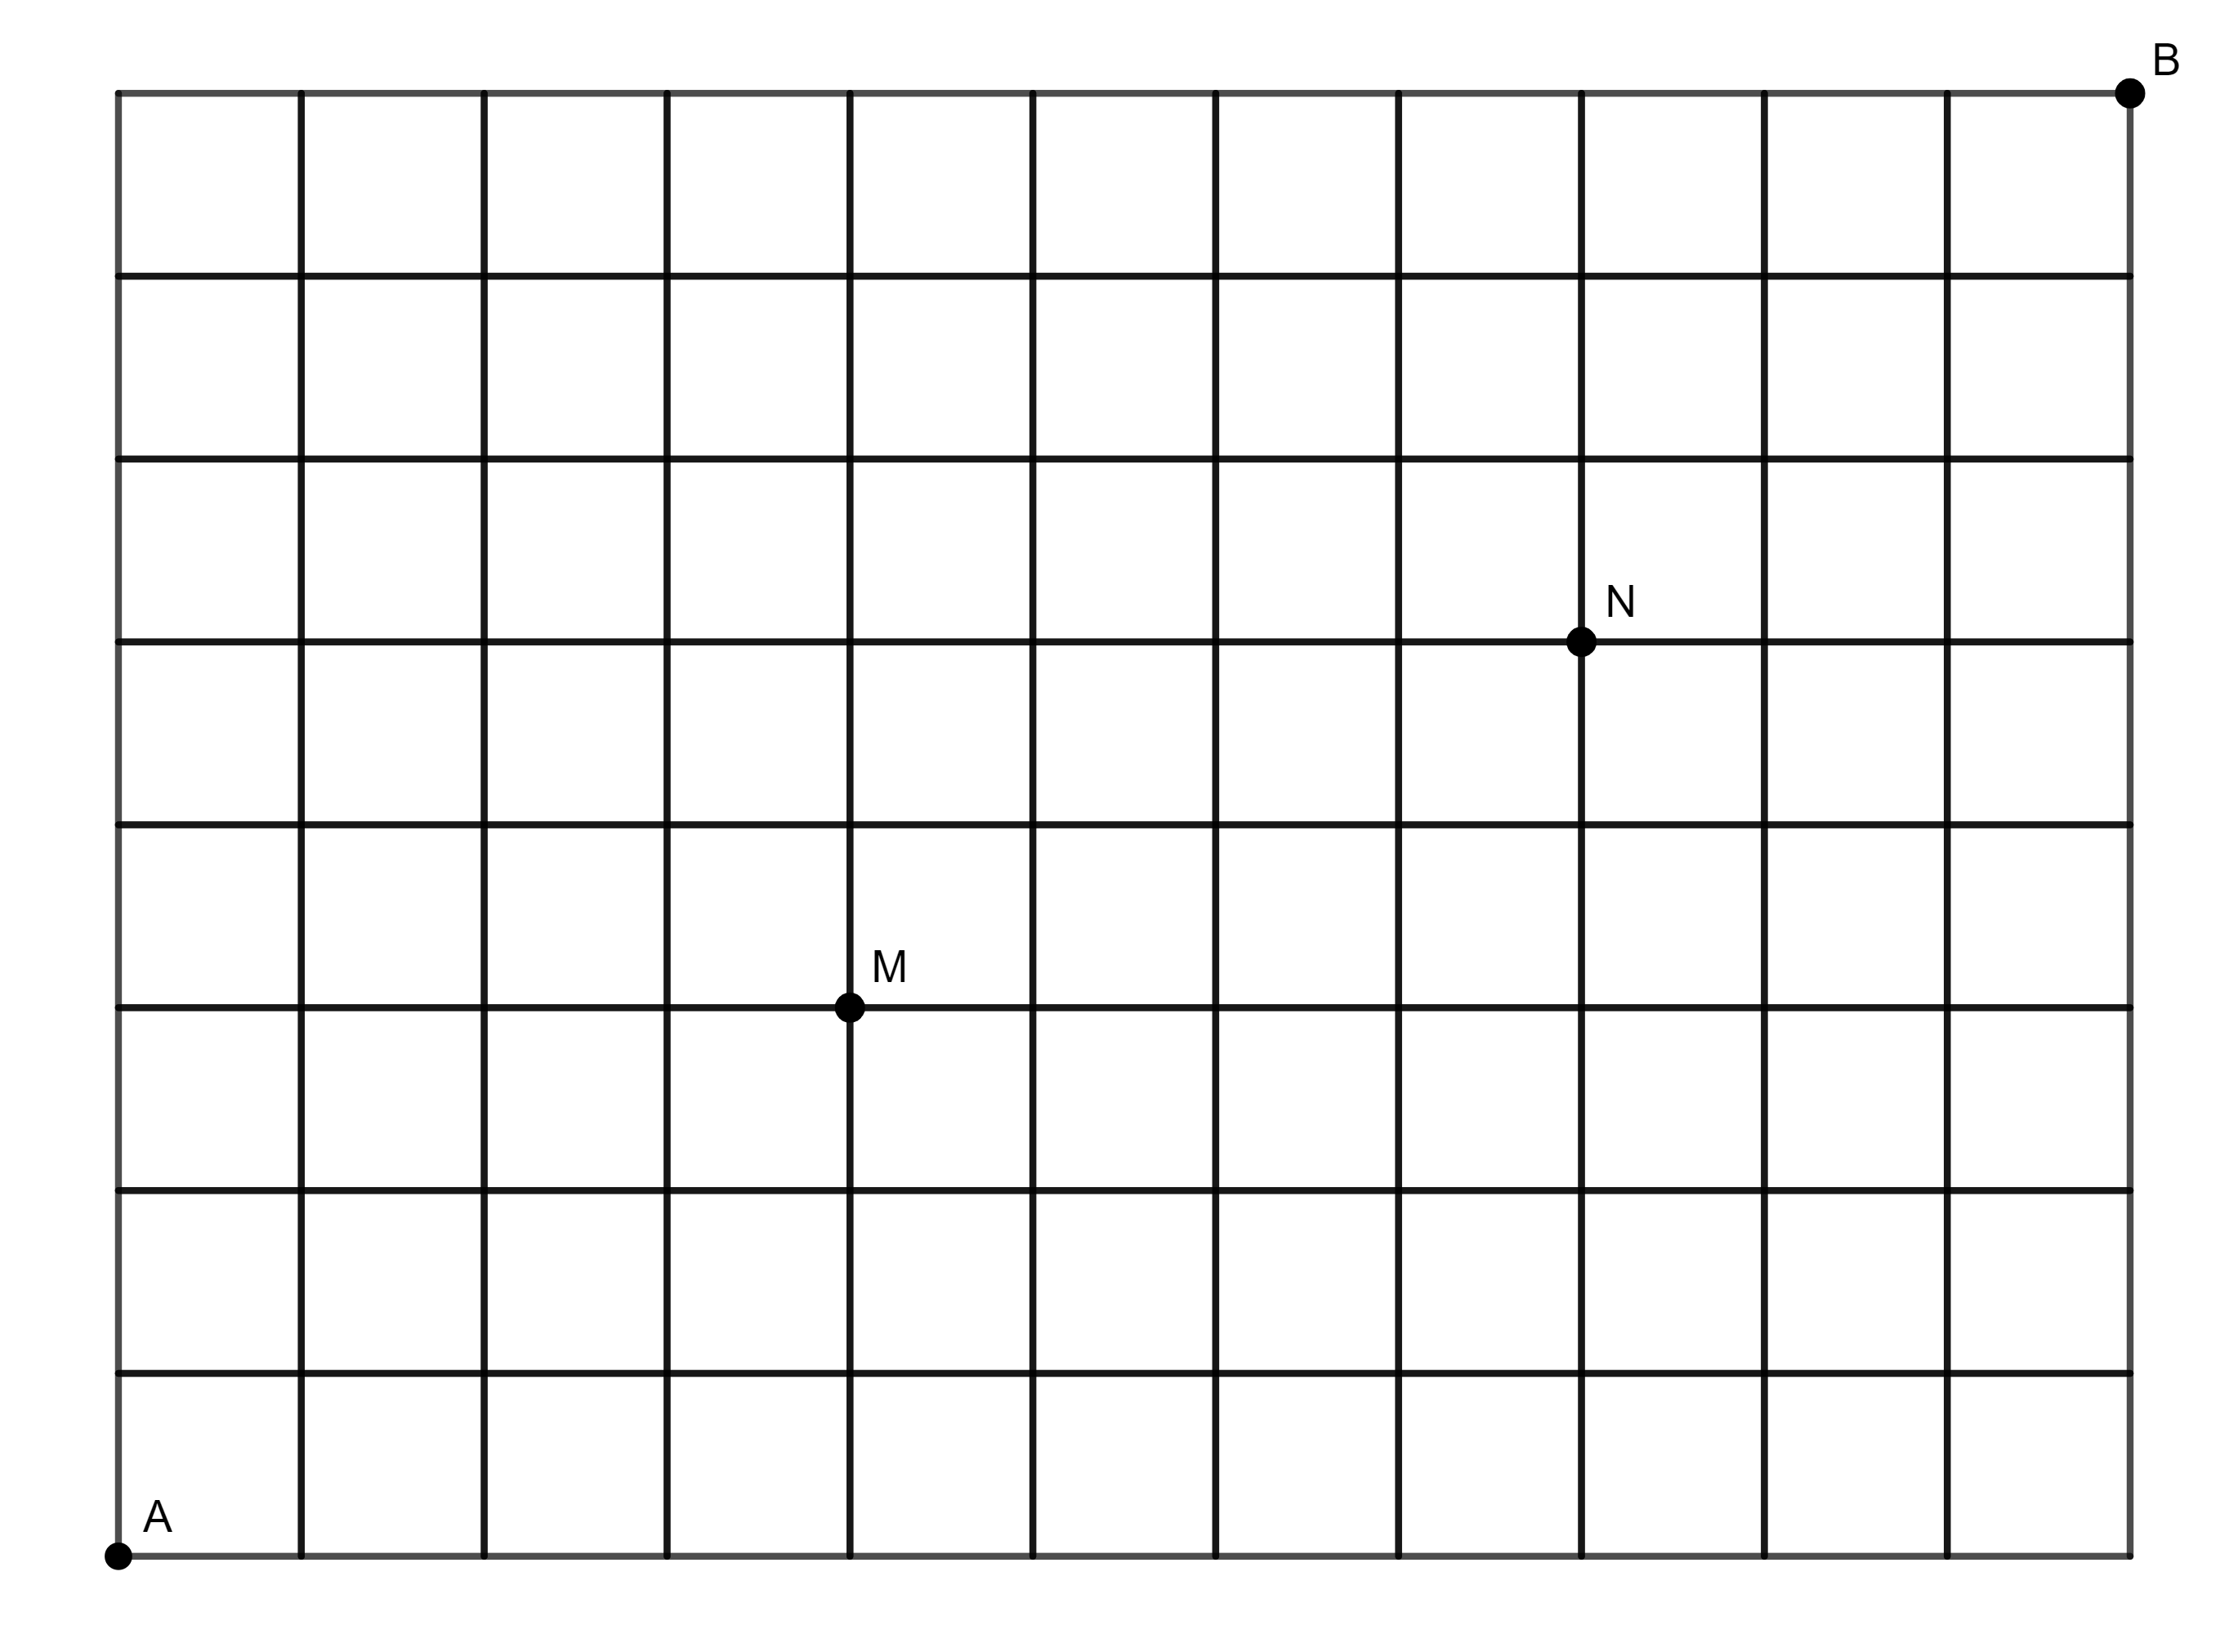
\includegraphics[scale=1]{Imagenes/IMG3/Caminos.png}
    \end{center}

    \renewcommand{\labelenumi}{\alph{enumi})}
    \begin{enumerate}
        \item De A a B.
        \item De A a M.
        \item De M a N.
        \item De A a B pasando por M.
        \item De A a B pasando por N.
        \item De A a B pasando por M y N.
        \item De A a B pasando por M o N.
        \item De A a B y no pasan ni por M ni por N.
        \item De A a B sin pasar por ningún punto de la última línea vertical (excepto B).
        \item De A a B pasando por un solo punto de de la segunda línea horizontal.
    \end{enumerate}
\end{problema}

\begin{problema}
    Una rana se ubica en el tercer escalón de unas gradas. La rana se mueve un escalón por salto (hacia arriba o hacia abajo). ¿Cuántas formas existen para que la rana llegue, en su noveno salto, al octavo escalón?
\end{problema}

\textbf{Crédito extra:} Se toma el elemento mayor de cada subconjunto de 7 elementos del conjunto $\{ 1,2,3,4,5,6,7,8,9,10 \}$. ¿Cuál es la suma de todos esos elementos mayores?

\end{document}